\chapter{更厉害的微分方程}
\section{用级数解微分方程}
前面说过,“好看”的函数可以展开成(泰勒)级数:$f(x)=\sum_{i=0}^{\infty} a_i x^i=a_0+a_1 x+a_2 x^2+\dots$,如果把级数代入微分方程,可以确定系数$a_i$,从而确定这个函数。

比如解方程$y''+y=0$(你应该能背出它的通解),把级数代进去得到
\begin{align*}
\sum_{i=2}^{\infty} (i-1)i a_i x^{i-2}+\sum_{i=0}^{\infty} a_i x^i&=0 \\
\sum_{i=0}^{\infty} (i+1)(i+2) a_{i+2} x^i+\sum_{i=0}^{\infty} a_i x^i&=0 \\
\sum_{i=0}^{\infty} ((i+1)(i+2) a_{i+2}+a_i) x^i=0
\end{align*}

这个式子对任何$x$都成立,所以每个$x^i$前面的系数都必须是$0$,也就是
\begin{equation*}
a_2=-\frac{1}{1 \cdot 2} a_0, a_4=-\frac{1}{3 \cdot 4} a_2, a_6=-\frac{1}{5 \cdot 6} a_4, \dots
\end{equation*}
\begin{equation*}
a_3=-\frac{1}{2 \cdot 3} a_1, a_5=-\frac{1}{4 \cdot 5} a_3, a_7=-\frac{1}{6 \cdot 7} a_5, \dots
\end{equation*}

写成通项就是
\begin{equation*}
a_n=\begin{cases}
\frac{1}{n!} a_0, &n \bmod 4=0 \\
\frac{1}{n!} a_1, &n \bmod 4=1 \\
-\frac{1}{n!} a_0, &n \bmod 4=2 \\
-\frac{1}{n!} a_1, &n \bmod 4=3
\end{cases}
\end{equation*}

到目前为止还没有确定$a_0$和$a_1$,它们需要用边界条件确定。前面说过,二阶微分方程的通解肯定有两个待定的参数。

把含$a_0$和$a_1$的项分开,可以发现它们就是$a_0 \cos x$和$a_1 \sin x$,因为前面说过
\begin{align*}
\sin x&=\sum_{n=0}^{\infty}\frac{1}{(2n+1)!}x^{2n+1}=x-\frac{1}{6}x^3+\frac{1}{120}x^5+\dots \\
\cos x&=\sum_{n=0}^{\infty}\frac{1}{(2n)!}x^{2n}=1-\frac{1}{2}x^2+\frac{1}{24}x^4+\dots
\end{align*}

但是,一般情况下即使算出了级数,找到原来的函数也不是一件容易的事情,需要摸索,需要练习。比如级数$\sum_{n=0}^{\infty} (-1)^n \frac{1}{2n+1} x^{2n+1}=x-\frac{1}{3} x^3+\frac{1}{5} x^5-\dots$,它就是$\frac{\pi}{2}-\arctan \frac{1}{x}$,你能想到吗?

【练习】解方程$y'+y=\rme^{-x}$。

如果已知一个函数,但是不容易把它展开成级数,可以反过来构造一个微分方程来算出级数。比如$y=\rme^{-\frac{1}{2} x^2}$,它满足$y'+x y=0$。把级数代进去得到
\begin{align*}
\sum_{i=1}^{\infty} i a_i x^{i-1}+\sum_{i=0}^{\infty} a_i x^{i+1}&=0 \\
\sum_{i=0}^{\infty} (i+1) a_{i+1} x^i+\sum_{i=1}^{\infty} a_{i-1} x^i&=0 \\
a_1+\sum_{i=1}^{\infty} ((i+1) a_{i+1}+a_{i-1}) x^i&=0
\end{align*}
\begin{equation*}
a_i=\begin{cases}
0, &i=1 \\
-\frac{1}{i} a_{i-2}, &i \ge 2
\end{cases}
\end{equation*}

写成通项就是$a_n=(-\frac{1}{2})^{\frac{n}{2}} \frac{1}{(\frac{n}{2})!} a_0 (n \text{为偶数})$,$n$为奇数时$a_n=0$,$a_0$仍然需要用边界条件确定。这样算比直接求导简单一些。

【练习】把$\rme^{\sin x}$表示成级数。
\section{狄拉克函数$\delta(x)$}
现在介绍一个奇怪的函数:$\delta(x)=\begin{cases} \infty, &x=0 \\ 0, &x \neq 0 \end{cases}$

这样并没有说清楚这个$\infty$是什么意思,我们知道无穷大也有大小之分,一般要通过极限来定义,虽然这里的定义方法不同。加上一条规定之后,$\delta(x)$的定义才算完整:对任何“好看”的函数$f(x)$,$\int_{-\infty}^{\infty} f(x) \delta(x) \opd x=f(0)$。

(看起来我要用“好看”这个词糊弄大家很久,我现在还不想讲紧支集之类太抽象的概念)

最平凡的情况是$f(x)=1$,也就是$\int_{-\infty}^{\infty} \delta(x) \opd x=1$。$\delta(x)$的图像大致如图\ref{fig-delta-x},但是图中的峰应该是无限细、无限高的,而且下面的面积为$1$,还要注意它是偶函数。
\begin{figure}[htb]
\centering
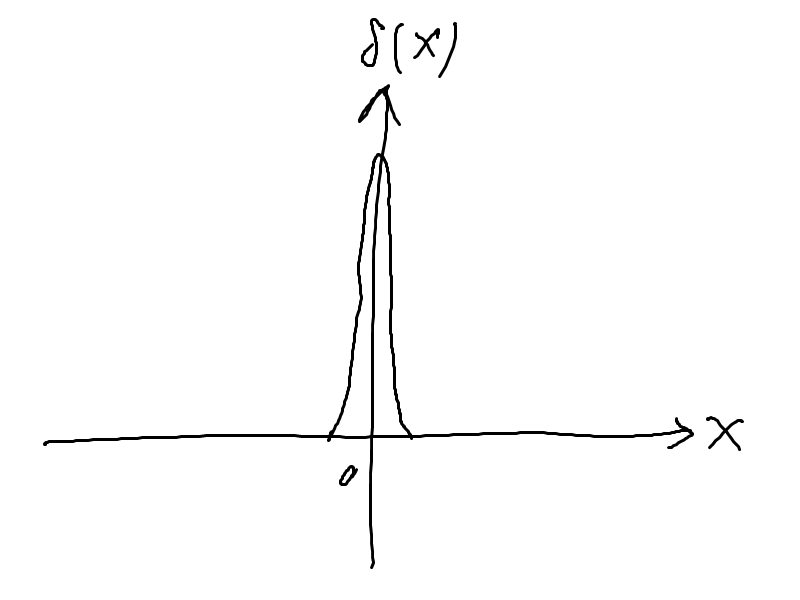
\includegraphics[scale=0.5]{fig/delta-x.png}
\caption{看起来尖尖的}
\label{fig-delta-x}
\end{figure}

物理学中的质点、点电荷之类体积无限小的东西可以用$\delta(x)$描述。比如一维空间中有一个质量为$10$,位置为$x=5$的质点,它的质量线密度$\lambda$(单位长度上的质量)可以表示为$\lambda(x)=10 \delta(x-5)$。你可以自己想一想三维空间中$\delta$函数的定义。

用极限来定义$\delta(x)$也是可以的。比如先定义$\delta_a(x)=\begin{cases} \frac{1}{2 a}, &-a \le x \le a \\ 0, &x<-a \text{或} x>a \end{cases}$,$a$是一个参数。$a \rightarrow 0$时,$\delta_a(x) \rightarrow \delta(x)$。除了这样的“方块”函数,也可以用其他类型的函数来定义,比如$\frac{\sin a x}{\pi x}$。可以证明,这些方法定义的是同一个$\delta(x)$。

(其实$\delta(x)$不是普通的函数,而是一种\emph{广义函数}。它在$x=0$时没有确定的值,跟高中课本对函数的定义不一样。至于什么叫“同一个”函数也有严格的定义)

$\delta(x)$可以求导和积分,一般令$\theta(x)=\int_{-\infty}^x \delta(t) \opd t$,称为单位阶跃函数或者赫维赛德$\theta$函数(传说是因为theta和step谐音)。$\delta'(x)$和$\theta(x)$如图\ref{fig-delta-d-x},你可以自己想一想更高阶的导数和积分的样子。物理学中的电偶极子可以用$\delta'(x)$描述。
\begin{figure}[htb]
\centering
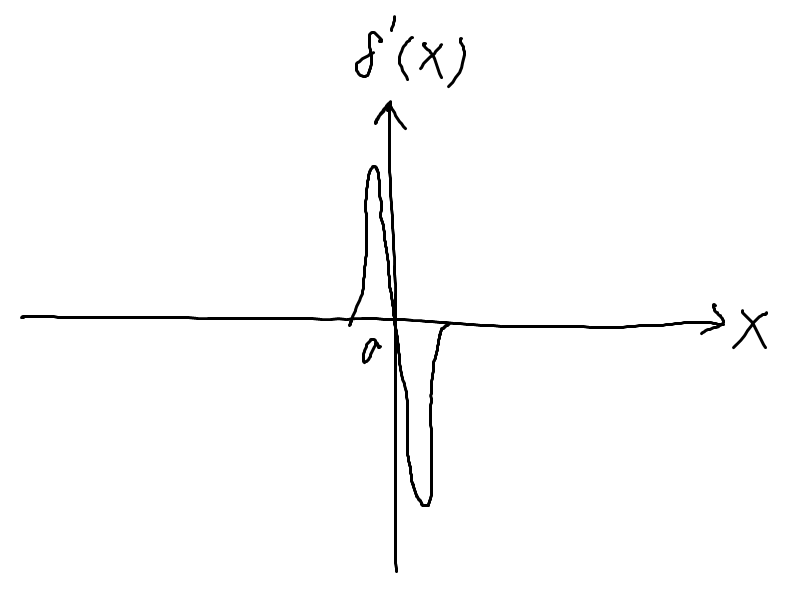
\includegraphics[scale=0.5]{fig/delta-d-x.png}
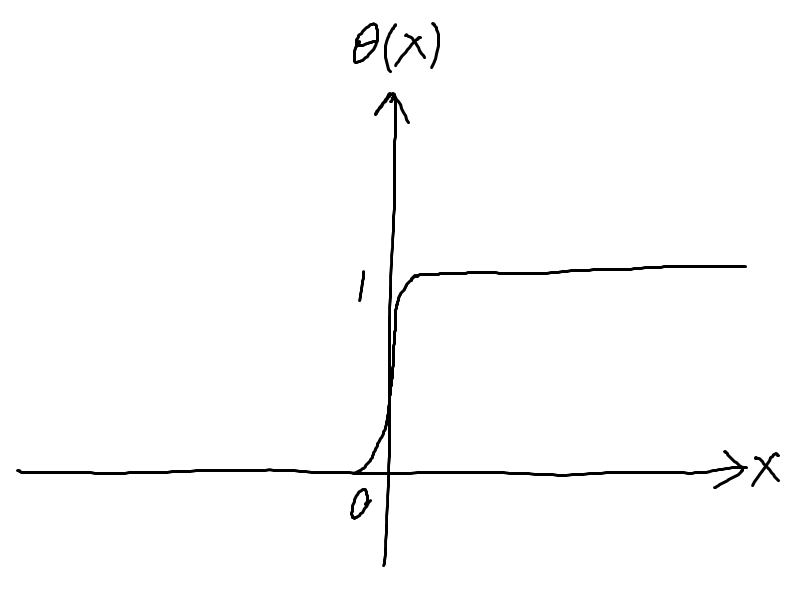
\includegraphics[scale=0.5]{fig/theta-x.png}
\caption{$\delta'(x)$和$\theta(x)$}
\label{fig-delta-d-x}
\end{figure}

现在断掉的分段函数也可以求导了,只要断点两边的距离是有限的,而不是爆掉。比如
\begin{equation*}
f(x)=\begin{cases}
x, &x<2 \\
x^3, &x>2
\end{cases} \Rightarrow f'(x)=\begin{cases}
1, &x<2 \\
6 \delta(x-2), &x=2 \\
3x^2, &x>2
\end{cases}
\end{equation*}

也就是说,$x$经过2的时候,$f(x)$经过了大小为$6$的突变。继续求导还可以得到
\begin{equation*}
f''(x)=\begin{cases}
0, &x<2 \\
6 \delta'(x-2)+11 \delta(x-2), &x=2 \\
6x, &x>2
\end{cases}
\end{equation*}

所以现在我们认为,断掉的函数在断点处也可以无限次求导或者积分。如果断点没有爆掉,求导或者积分之后也不会爆掉。

矢量分析那里讲过的克罗内克张量$\delta_{i j}=\begin{cases} 1, &i=j \\ 0, &i \neq j \end{cases}$与这里的$\delta(x)$有相似之处。
\section{用格林函数解微分方程}
现在还是来解关于$y(x)$的方程$y''+y=f(x)$。如果把$y$看成弹簧振子的位置,$x$看成时间,它可以表示无阻尼的弹簧振子($k=m=1$),$f(x)$表示外力。

如果$f(x)=\delta(x)$,表示$x=0$时戳它一下,给弹簧振子一个冲量。如果之前它是静止的,之后速度突变为$1$。(至于之前是不是静止要看通解,这里先不考虑)

可以猜出方程的特解为$y=\theta(x) \sin(x)$,也就是说$x=0$之前弹簧振子不动,之后作振幅为$1$的简谐振动,这符合我们的直觉。

如果要验证这个解是对的,可以先算出$y''=\delta'(x) \sin(x)+2 \delta(x) \cos(x)-\theta(x) \sin(x)$,然后代入方程,只需证明$\delta'(x) \sin(x)+2 \delta(x) \cos(x)=\delta(x)$。

按照$\delta(x)$的定义,这时必须把方程两边与任意的$g(x)$相乘($f(x)$被用掉了),然后对$x$积分:
\begin{align*}
\int_{-\infty}^{\infty} \delta'(x) \sin(x) g(x) \opd x+2 \int_{-\infty}^{\infty} \delta(x) \cos(x) g(x) \opd x&=\int_{-\infty}^{\infty} \delta(x) g(x) \opd x
\end{align*}

按照定义,右边为$g(0)$。如果把$\cos(x) g(x)$看成一个函数,那么左边第二项就是$2 g(0)$,只需证明左边第一项为$-g(0)$。用分部积分把$\delta'(x)$变成$\delta(x)$:
\begin{align*}
\int_{-\infty}^{\infty} \delta'(x) \sin(x) g(x) \opd x&=\delta(x) \sin(x) g(x)|_{-\infty}^{\infty}-\int_{-\infty}^{\infty} \delta(x) \ddx(\sin(x) g(x)) \opd x \\
&=-\int_{-\infty}^{\infty} \delta(x) \cos(x) g(x) \opd x-\int_{-\infty}^{\infty} \delta(x) \sin(x) g'(x) \opd x
\end{align*}

这里的第一项是$-g(0)$,第二项是$0$,所以上面的式子成立。

如果$f(x)=\delta(x)+2 \delta(x-1)$,可以猜出特解$y=\theta(x) \sin(x)+2 \theta(x-1) \sin(x-1)$。也就是说,$x=0$时戳一下,$x=1$时更重地戳一下,两者的效果可以线性叠加。为了方便,令$G(x)=\theta(x) \sin(x)$,$y=G(x)+2 G(x-1)$。

现在神奇的事情来了:任何$f(x)$可以看作无穷多个不同高度的$\delta$函数的叠加,也就是$f(x)=\int_{-\infty}^{\infty} f(t) \delta(x-t) \opd t$,如图\ref{fig-many-delta}。比如$t=1$时,要放一个$\delta(x-1)$,高度为$f(1)$。这样一来,可以直接写出特解$y(x)=\int_{-\infty}^{\infty} f(t) G(x-t) \opd t$。
\begin{figure}[htb]
\centering
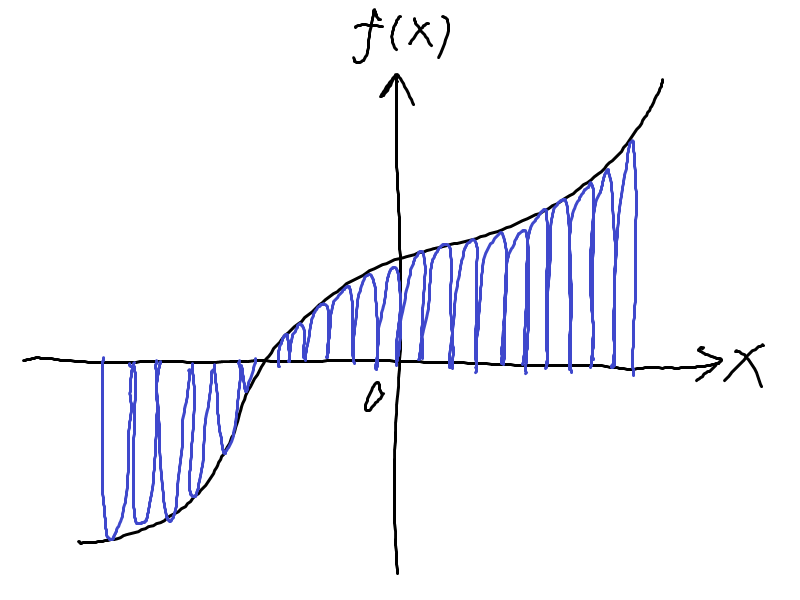
\includegraphics[scale=0.5]{fig/many-delta.png}
\caption{戳得多了就变光滑了}
\label{fig-many-delta}
\end{figure}

举个栗子:外力从$x=0$开始线性变化,$f(x)=\theta(x) x=\begin{cases} 0, &x<0 \\ x, &x>0 \end{cases}$。

(如果没有$\theta(x)$,$x \rightarrow -\infty$时$y$的情况就无法确定,也就是没有好的边界条件)
\begin{align*}
y(x)&=\int_{-\infty}^{\infty} \theta(t) t \cdot \theta(x-t) \sin(x-t) \opd t \\
&=\int_{0}^{x} t \sin(x-t) \opd t \\
&=x-\sin x
\end{align*}

也就是说,弹簧振子的运动是匀速直线运动和简谐振动的叠加。当然这是特解,不要忘了加上对应的齐次方程的通解。

$G(x)$是方程$y''+y=f(x)$在$f(x)=\delta(x)$时的特解,称为格林函数,也有些地方称为积分核、瞬态响应之类的。它的好处在于,只要在$f(x)=\delta(x)$时想办法解出微分方程,其他奇怪的$f(x)$不用另外想办法,可以直接转化为积分。至于这个积分能不能积出来,仍然不是我们现在关心的事情。

要强调的是,格林函数利用了解的线性叠加,因此只对线性非齐次微分方程适用(不一定是常系数)。

不同的方程有不同的格林函数,比如阻尼振动$y''+2 \beta y'+y=f(x)$,
\begin{equation*}
G(x)=\theta(x) \frac{e^{-(\beta+\sqrt{\beta^2-1}) x}-e^{-(\beta-\sqrt{\beta ^2-1}) x}}{2 \sqrt{\beta^2-1}}
\end{equation*}

既然你看过前面的内容,这个解也很容易猜出来,就是阻尼振动的通解代入初始位置为$0$、速度为$1$的条件,再乘上$\theta(x)$。用这个$G(x)$算积分一看就很麻烦,这里只能给大家大概地讲一讲解微分方程的方法,当然手算积分的功底也很重要,需要刷足够多的题才能练出来。

【练习】解方程$y'+y=\theta(x) x^2$。想一想刚才的步骤:猜出格林函数,验证,算出积分,最后别忘了加上通解。
\section{傅立叶变换的性质}
这一章用的傅立叶变换公式是
\begin{equation*}
g(k)=\mathscr{F}_{x \rightarrow k} f(x)=\frac{1}{\sqrt{2 \pi}} \int_{-\infty}^{\infty} f(x) \rme^{-\rmi k x} \opd x, f(x)=\mathscr{F}^{-1}_{x \rightarrow k} g(k)=\frac{1}{\sqrt{2 \pi}} \int_{-\infty}^{\infty} g(k) \rme^{\rmi k x} \opd k
\end{equation*}

傅立叶变换是线性的,跟积分的性质差不多,$\mathscr{F}(a_1 f_1+a_2 f_2)=a_1 \mathscr{F} f_1+a_2 \mathscr{F} f_2$。

通过换元还可以证明$\mathscr{F}_{x \rightarrow k} f(x+a)=\rme^{\rmi k a} \mathscr{F}_{x \rightarrow k} f(x)$,$\mathscr{F}_{x \rightarrow k} f(a x)=\frac{1}{a} \mathscr{F}_{x \rightarrow \frac{k}{a}} f(x)$,$a$是常量。

先对$f(x)$求导再进行傅立叶变换会怎么样呢?
\begin{align*}
\mathscr{F}_{x \rightarrow k} \ddx f(x)&=\frac{1}{\sqrt{2 \pi}} \int_{-\infty}^{\infty} \frac{\opd f(x)}{\opd x} \rme^{-\rmi k x} \opd x \\
&=\frac{1}{\sqrt{2 \pi}} \int_{-\infty}^{\infty} \rme^{-\rmi k x} \opd f(x) \\
&=-\frac{1}{\sqrt{2 \pi}} \int_{-\infty}^{\infty} f(x) \opd \rme^{-\rmi k x}
\internote{(这里用了分部积分,应该还有一项$\left. f(x) \rme^{-\rmi k x} \right|_{-\infty}^{\infty}$。如果$f(\pm \infty)=0$,那么这一项就是0,但是以后在这里会遇到一些问题)}
&=\rmi k \frac{1}{\sqrt{2 \pi}} \int_{-\infty}^{\infty} f(x) \rme^{-\rmi k x} \opd x \\
&=\rmi k \mathscr{F}_{x \rightarrow k} f(x)
\end{align*}

所以傅立叶变换可以把求导变成乘$\rmi k$,在解微分方程的时候比较方便。以前我们猜$x(t)=x_0 \rme^{\rmi \omega t}$也是这个原因。

类似地有$\mathscr{F}_{x \rightarrow k} \int f(x) \opd x=\frac{1}{\rmi k} \mathscr{F}_{x \rightarrow k} f(x)+C \delta(k)$,$C \delta(k)$是对积分常量做傅立叶变换的结果,这个待会再讲。

$\delta(x-a)$的傅立叶变换是什么呢?$\mathscr{F}_{x \rightarrow k} \delta(x-a)=\frac{1}{\sqrt{2 \pi}} \int_{-\infty}^{\infty} \delta(x-a) \rme^{-\rmi k x} \opd x=\frac{1}{\sqrt{2 \pi}} \rme^{-\rmi a k}$。再进行逆变换:$\frac{1}{\sqrt{2 \pi}} \int_{-\infty}^{\infty} \frac{1}{\sqrt{2 \pi}} \rme^{-\rmi a k} \rme^{\rmi k x} \opd k=\delta(x)$。

也就是说,$\int_{-\infty}^{\infty} \rme^{\rmi k (x-a)} \opd k=2 \pi \delta(x-a)$。如果直接计算这个积分,会得到$\frac{1}{\rmi (x-a)} \rme^{\rmi k (x-a)}$,$k \rightarrow \pm \infty$时它是没有定义的。但是借助$\delta(x)$,我们就是把它算出来了。

现在来看看常函数$f(x)=1$的傅立叶变换:$\mathscr{F}_{x \rightarrow k} 1=\frac{1}{\sqrt{2 \pi}} \int_{-\infty}^{\infty} \rme^{-\rmi k x} \opd x=\sqrt{2 \pi} \delta(k)$。

想一想傅立叶变换的物理意义,它把函数变成频谱。如果把$f(x)$看成无穷多个复振动$A_k \rme^{\rmi k x}$的叠加,变换出来的$g(k)$表示频率为$k$的振动的强度。常函数$f(x)=1$里面没有这样的振动,所以只有$k=0$时$g(k) \neq 0$,否则$g(k)=0$。至于系数$\sqrt{2 \pi}$没有这么显然,但是用上面的方法可以算出来。

一个三角函数相当于两个复振动:$\sin a x=\frac{1}{2 \rmi}(\rme^{\rmi a x}-\rme^{-\rmi a x})$,$\cos a x=\frac{1}{2}(\rme^{\rmi a x}+\rme^{-\rmi a x})$。现在可以直接看出$\mathscr{F}_{x \rightarrow k} \sin a x=-\rmi \sqrt{\frac{\pi}{2}} (\delta(k-a)-\delta(k+a))$,$\mathscr{F}_{x \rightarrow k} \cos a x=\sqrt{\frac{\pi}{2}} (\delta(k-a)+\delta(k+a))$。
\section{用傅立叶变换解微分方程}
现在又要解方程$y''+y=\sin a x$。对两边同时进行傅立叶变换:$(-k^2+1) Y=-\rmi \sqrt{\frac{\pi}{2}} (\delta(k-a)-\delta(k+a))$,其中$Y(k)=\mathscr{F}_{x \rightarrow k} y(x)$。

可以直接算出$Y=\rmi \sqrt{\frac{\pi}{2}} \frac{\delta(k-a)-\delta(k+a)}{1-k^2}$,然后用傅立叶逆变换就能算出$y$。含有$\delta(x)$的积分都比较好算,比如$\int_{-\infty}^{\infty} \frac{\delta(k-a)}{1-k^2} \rme^{\rmi k x} \opd k=\frac{\rme^{\rmi a x}}{1-a^2}$。逆变换的结果是
\begin{align*}
y&=\frac{1}{\sqrt{2 \pi}} \int_{-\infty}^{\infty} -\rmi \sqrt{\frac{\pi}{2}} \frac{\delta(k-a)-\delta(k+a)}{1-k^2} \rme^{\rmi k x} \opd k \\
&=-\frac{\rmi}{2} \int_{-\infty}^{\infty} \frac{\delta(k-a)-\delta(k+a)}{1-k^2} \rme^{\rmi k x} \opd k \\
&=-\frac{\rmi}{2} \frac{\rme^{\rmi a x}-\rme^{\rmi a x}}{1-a^2} \\
&=\frac{\sin a x}{1-a^2}
\end{align*}

跟以前受迫振动的结果一样,振动频率就是外力的频率$a$,而系统的本征频率是$1$。$a$离$1$越近,振幅就越大,$a=1$时就会爆掉。

仍然别忘了这是特解,还要加上通解。如果只有齐次方程$y''+y=0$,傅立叶变换之后就是$(-k^2+1) Y=0$。$k \neq 0$时$Y=0$,$k=0$时$Y$可以是任意值,所以通解是$y=A \sin x+B \cos x$。

【练习】解方程$y''+y=\sin 2 x+\cos 3 x+\sin 4 x$,想一想频谱的叠加是什么样的。

$\phantom{\text{【练习】}}$解方程$y''+y'+y=\sin a x$。

如果外力的频谱已知或者容易求出,那就适合用傅立叶变换来解方程。还有一种类似的变换叫拉普拉斯变换,这里就不讲了。
